\section{Theoretical results}
\label{sec:theory}

We derive an analytical model for the localization dynamics of the single-neuron architecture in \labelcref{item:single-neuron-model}.
This result establishes necessary and sufficient conditions for localization under Properties~\labelcref{item:weak-dependence,item:translation-invariance,item:sign-symmetry} for the minimal case of a binary response, \ie $y = 0,1$.
The conditions for localization in the single-neuron architecture in \labelcref{item:single-neuron-model} are demonstrated in \cref{sec:experiments} to also hold empirically for the many-neuron architecture in \labelcref{item:many-neuron-model}.
Further, we use this model to derive a negative prediction about localization, that the architectures in \labelcref{item:many-neuron-model,item:single-neuron-model} fail to learn a localized receptive field on elliptical distributions
despite their non-Gaussian---in particular, significantly positive kurtosis---statistics~\parencite[\cf positive kurtosis as an objective or diagnostic for localization,][]{hyvarinen2000independent,ingrosso2022data}.

\subsection{An analytical model for the dynamics of localization in a single neuron}

Previous approaches to obtain analytical dynamics in the architectures in 
\labelcref{item:many-neuron-model,item:single-neuron-model} 
have studied the gradient flow under the assumption that the preactivation $\langle \mathbf{w}, \mathbf{X} \rangle$ is approximately Gaussian~\parencite{goldt2020modelling,gerace2020generalisation,goldt2022gaussian}, but this assumption fails to capture the propagation of higher-order statistics through a neural network that promotes localization~\cite{ingrosso2022data}.
Happily, the idealized visual input setting set out in \labelcref{item:weak-dependence,item:translation-invariance,item:sign-symmetry} permits us some simplification.
In particular, 
the translation-invariance of the data $\mathbf{X}$ under \labelcref{item:translation-invariance} and 
the architecture of \labelcref{item:single-neuron-model}
allow us to work with the marginal distributions of each input dimension, $X_i$ rather than the full joint distribution of $\mathbf{X}$.

We now give the analytical simplifications that allow us to derive an analytical model for the localization dynamics of the single neuron architecture in \labelcref{item:single-neuron-model}, namely
two assumptions on $\mathbf{X} \mid X_i$ for all $i \in \{1, \dots, N\}$ as a well as a mild condition on the weights that is satisfied at initialization.
These are, where $\sigma_i^y$ to denotes the $i$-th row of $\Sigma_y$:

\newcounter{assumenumi}
\begin{analysis}{\textbf{Analytical simplifications 1--3} (\emph{early-time, limiting dynamics}).}{}
\begin{enumerate}[series=assumenumi]
  \item \label{item:mean-assumption} $\E[\mathbf{X} \mid X_i = x_i, Y = y] = x_i \sigma_i^y$, \ie the conditional mean scales linearly with $x_i$.
  \item \label{item:covariance-assumption} $\text{Cov}[\mathbf{X} \mid X_i = x_i, Y = y] = \Sigma_y - \sigma_i^y \sigma_i^{y\top}$, \ie the conditional covariance is smaller near $i$, but independent of the exact value of $x_i$.
  \item \label{item:lindeberg-condition} Lindeberg's condition holds for the sequence $w_1 X_1, \ldots, w_N X_N \mid X_i = x_i$ as $N \to \infty$ for all $x_i$.
\end{enumerate}
\end{analysis}

Our motivation for Assumptions~\labelcref{item:mean-assumption,item:covariance-assumption,item:lindeberg-condition} is that they replicate the kurtosis of the marginal distributions $X_i$ (discussed further below) of two important and distinct limiting cases where localization does and does not appear, respectively:
when $\mathbf{X}$ has support on the vertices of the hypercube $\{ \pm 1 \}^N$ (satisfied by \texttt{Ising} for any $J$), and
when $\mathbf{X}$ is Gaussian (satisfied by \texttt{NLGP} with $g \approx 0$).

The gradient flow in Lemma~\labelcref{lem:gradient_flow} also relies on Assumption~\labelcref{item:lindeberg-condition} that Lindeberg's condition holds for the sequence $w_i X_i$, which ensures that no single term $w_i X_i$ in the sequence can dominate.
If this holds, then we can conclude that $\langle \mathbf{w}, \mathbf{X} \rangle \mid X_i$ is approximately Gaussian.
As we discuss in \cref{subsec:pf_of_gradient_flow}, this is almost always satisfied for a Gaussian initialization of $\mathbf{w}$, and for slight deviations therefrom, and is satisfied by the settings of \textcite{ingrosso2022data}.
Using this fact, we obtain an explicit form for the gradient flow early in training, stated in Lemma~\labelcref{lem:gradient_flow}.

\begin{lemma} \label{lem:gradient_flow}
    Under Assumptions~\labelcref{item:mean-assumption,item:covariance-assumption},
    the gradient flow for the single ReLU neuron in \labelcref{item:single-neuron-model} early in training with $y = 0, 1$ 
    trained using MSE loss is
    \begin{equation} \label{eq:gradient_flow_early}
      \frac{2}{\tau} \frac{\mathrm{d}\mathbf{w}}{\mathrm{d}t} = \varphi\left( \frac{\Sigma_1 \mathbf{w}}{\sqrt{\langle \Sigma_1 \mathbf{w}, \mathbf{w} \rangle}} \right) - ( \Sigma_0 + \Sigma_1 ) \mathbf{w} + o_N(1),
    \end{equation}
    where $o_N(1)$ vanishes as $N\to\infty$, and where $\varphi : (-1,1) \to \R$ is defined as
    \begin{equation} \label{eq:varphi}
        \varphi(a) = \E_{X_1 \mid Y = 1}\left[ X_1 \operatorname{erf}\left( X_1 \operatorname{alg}^{-1}(a) / \sqrt{2} \right)
        \right]
    \end{equation}
    and $\operatorname{alg}^{-1}(x) = x/\sqrt{1-x^2}$, the inverse of the algebraic sigmoid function $\operatorname{alg}(x) = x/\sqrt{1+x^2}$.
\end{lemma}
Lemma~\labelcref{lem:gradient_flow} reduces the study of higher-order statistics to the marginal distributions, $X_1$, where, by translation invariance, all marginals have the same distribution, so we refer to $X_1$ without loss of generality.
While Lemma~\labelcref{lem:gradient_flow} technically only holds early in training and breaks down if $\mathbf{w}$ becomes localized due to violation of \labelcref{item:lindeberg-condition}, the gradient flow in \cref{eq:gradient_flow_early} holds sufficiently long to detect the emergence of localization in the weights $\mathbf{w}$.
In particular, numerically integrating \cref{eq:gradient_flow_early} yields localized weights $\mathbf{w}$ as $t \to \infty$.
Moreover, the location of the peak of final weights from \cref{eq:gradient_flow_early} corresponds closely to the actual peak of the weight, when we observe localization; see \cref{sec:peak-prediction} 
for empirical validation of this fact.
The primary difference observed is that the localized bump from \cref{eq:gradient_flow_early} is less peaked than when computed exactly; see \cref{fig:theory} for a comparison between experimentally observed localized receptive fields and theoretical predictions.

\subsection{Necessary and sufficient conditions for emergent localization}
\label{subsec:localization_conditions}

To establish an exact threshold at which localization emerges requires solving \cref{eq:gradient_flow_early}, which is not possible exactly for general nonlinear differential equations.\smash{\footnotemark}\footnotetext{
We discuss a partial differential equation limit that faces similar intractabilities in \cref{sec:pde-limit}.
}
Nevertheless, the form of \cref{eq:gradient_flow_early} reveals that localization is driven solely by the first term. 
Indeed, the second term depends only on the second-order statistics of the data, and so can be held fixed as $\mathbf{X}$ is varied from a distribution that induces localization to one that does not.
Secondly, one can see that the first term in \cref{eq:gradient_flow_early} does not change as $\mathbf{w}$ is scaled, in contrast to the second term.
As such, the second term in \cref{eq:gradient_flow_early} serves to constrain the \emph{scale} of $\mathbf{w}$, distinct from localization, while the first is primarily concerned with the \emph{shape} of $\mathbf{w}$, and thus localization.
This further motivates the first term, and thus $\varphi$, 
which we will refer to as the \emph{amplifier} and which itself depends on properties of the data distribution $p(\mathbf{X})$,
as a focus of study for understanding localization.

\newcommand{\sampleheight}{42pt}
\newcommand{\covheight}{46pt}
\newcommand{\marginalheight}{50pt}
\setlength{\tabcolsep}{4pt}
\begin{figure}[t]
  \centering
  \hspace{-1.2em}
  \scalebox{0.9}{
  \begin{centering}
    \begin{tabular}{p{51pt}
      @{\hspace{10pt}}m{2pt}l
      @{\hspace{5pt}}l
      @{\hspace{10pt}}m{2pt}l
      @{\hspace{10pt}}m{2pt}l}
        \raisebox{18pt}{\small$\texttt{Ising}$} &
        \raisebox{34pt}{\rotatebox{90}{\tiny input value}} &
        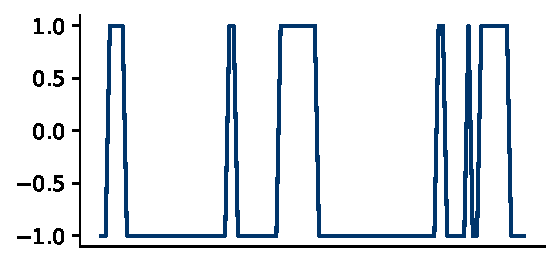
\includegraphics[height=\sampleheight]{figures/task/samples_long/ising.pdf} &
        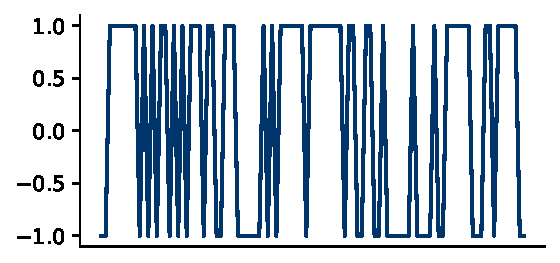
\includegraphics[height=\sampleheight]{figures/task/samples_short/ising.pdf} &
        \raisebox{38pt}{\rotatebox{90}{\tiny input dimension}} &
        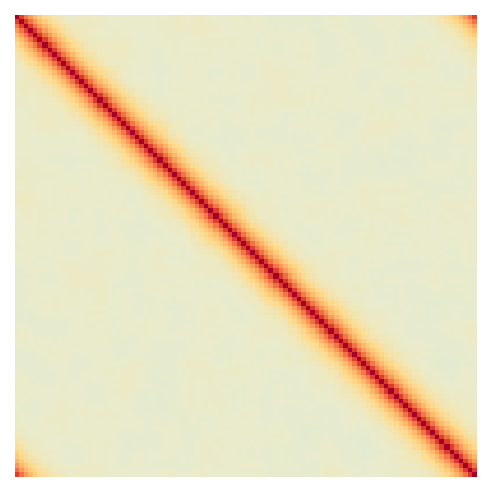
\includegraphics[height=\covheight]{figures/task/cov/ising.pdf} &
        \raisebox{40pt}{\rotatebox{90}{\tiny $p(X_i)$}} &
        \raisebox{-4pt}{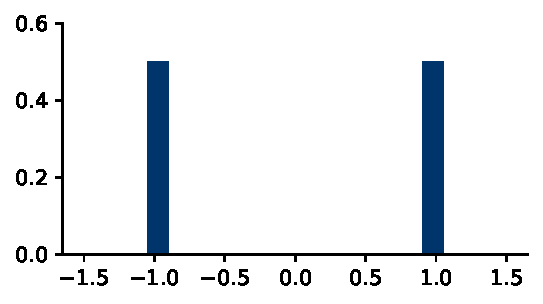
\includegraphics[height=\marginalheight]{figures/task/marginal/ising.pdf}} \\
        \noalign{\vskip -36pt}
        \raisebox{18pt}{\small$\texttt{NLGP}(0.01)$} &
        \raisebox{34pt}{\rotatebox{90}{\tiny input value}} &
        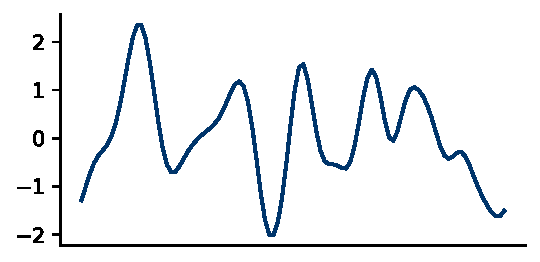
\includegraphics[height=\sampleheight]{figures/task/samples_long/gaussian.pdf} &
        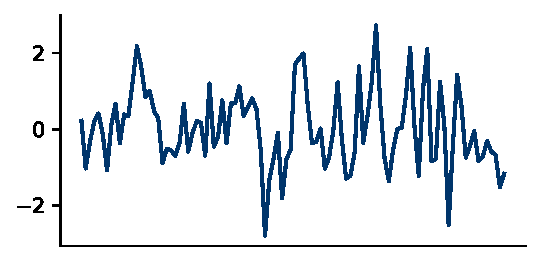
\includegraphics[height=\sampleheight]{figures/task/samples_short/gaussian.pdf} &
        \raisebox{38pt}{\rotatebox{90}{\tiny input dimension}} &
        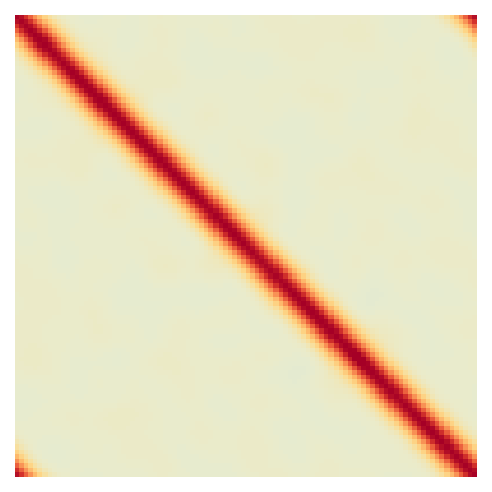
\includegraphics[height=\covheight]{figures/task/cov/gaussian.pdf} &
        \raisebox{40pt}{\rotatebox{90}{\tiny $p(X_i)$}} &
        \raisebox{-4pt}{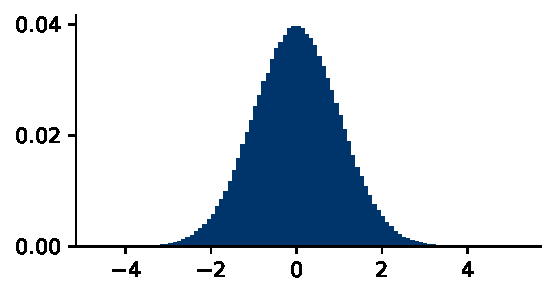
\includegraphics[height=\marginalheight]{figures/task/marginal/gaussian.pdf}} \\
        \noalign{\vskip -36pt}
        \raisebox{18pt}{\small $\texttt{Kur}(5)$} &
        \raisebox{34pt}{\rotatebox{90}{\tiny input value}} &
        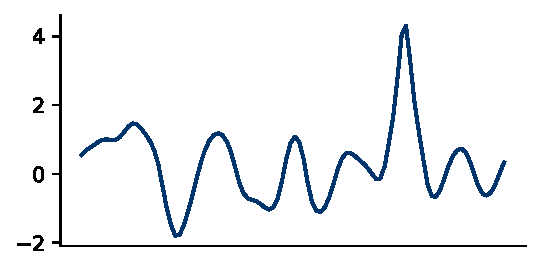
\includegraphics[height=\sampleheight]{figures/task/samples_long/alg5.pdf} &
        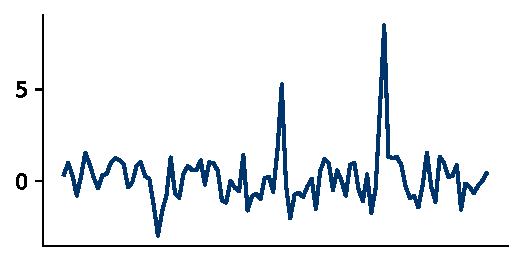
\includegraphics[height=\sampleheight]{figures/task/samples_short/alg5.pdf} &
        \raisebox{38pt}{\rotatebox{90}{\tiny input dimension}} &
        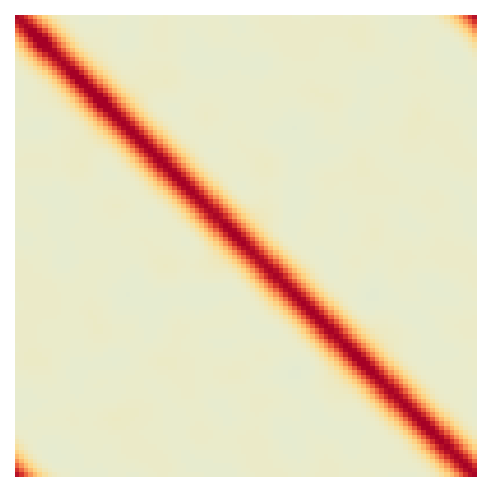
\includegraphics[height=\covheight]{figures/task/cov/alg5.pdf} &
        \raisebox{40pt}{\rotatebox{90}{\tiny $p(X_i)$}} &
        \raisebox{-4pt}{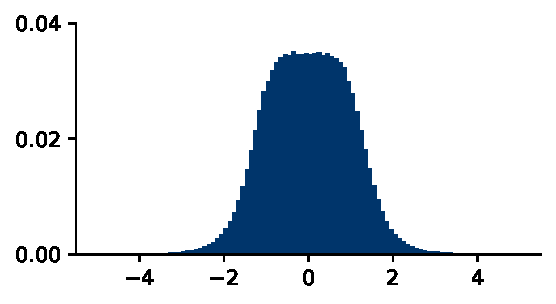
\includegraphics[height=\marginalheight]{figures/task/marginal/alg5.pdf}} \\
        \noalign{\vskip -37pt}
        &&
        \hspace{25pt}\tiny input dimension &
        \hspace{25pt}\tiny input dimension & &
        \hspace{3pt}\tiny input dimension & &
        \hspace{37pt}\tiny input value \\
  \end{tabular}
  \end{centering}
  }
  \caption{
    从左到右:
    长尺度和短尺度样本 $\mathbf{x}$,
    单一尺度的协方差 $\Sigma$,
    以及数据模型的边缘分布 $p(X_i)$,如 \cref{sec:task} 所述:
    Ising 模型(左、右样本分别为 $J=1.2, 0.3$),
    非线性高斯过程~\parencite[NLGP;~][]{ingrosso2022data},
    以及可控峰度模型 \texttt{Kur}
    (左、右样本分别为 $\xi=5, 1$)。
    \emph{
    每个模型生成的样本以零为中心,且其协方差可以被约束为相似,
    但具有不同的高阶统计量,从维度方向的边缘分布中可以看出这一点。
    }
}
  \label{fig:task}
  \vspace{-10pt}
\end{figure}


We present an analysis of $\varphi$ in \cref{sec:varphi-analysis} that reveals the role of the marginal distribution of the data in driving localization.
For each marginal, $\varphi(a) \approx (\sqrt{2/\pi}) a$ for $a \approx 0$.
For larger $a$, $\varphi$ depends more strongly on the data distribution and can be super-linear (sub-linear), \ie greater (smaller) than $(\sqrt{2/\pi}) a$.
Super-linear $\varphi$ encourage entries in $\mathbf{w}$ that are large in some neighborhood to grow faster than those that are smaller, yielding localization.
Linear and sub-linear $\varphi$ are the opposite, encouraging oscillatory or flat weights by suppressing neighborhoods in $\mathbf{w}$.
However, super- and sub-linearity may not hold uniformly, as $\varphi$ can be both  over its domain (see \cref{fig:theory}, bottom row, black line).
As an approximation, we consider a third-order Taylor expansion (red lines in \cref{fig:theory}, second column), which reveals that for the canonical setting of $\sigma^2 = 1$, \emph{negative excess kurtosis of the marginals yields super-linearity}, while \emph{positive excess kurtosis yields sub-linearity};
see \cref{sec:varphi-analysis}.
This leads us to the following claim, which is validated by our simulations in \cref{sec:experiments}:
\begin{claim} \label{thm:localization}
    For sufficiently large $N$, if the data $\mathbf{X} \in \R^N$ satisfies conditions \labelcref{item:weak-dependence,item:translation-invariance,item:sign-symmetry} and has marginal distributions with sufficiently \emph{negative} excess kurtosis, then Model~\labelcref{item:single-neuron-model} will learn localized receptive fields.
    Conversely, if the excess kurtosis is sufficiently \emph{positive}, it will not.
\end{claim}

As a minimal positive example, the distribution with the most negative excess kurtosis is the symmetric Bernoulli, with a value of $-2$.
In our setting, this corresponds to a data vector $\mathbf{X}$ with support on the vertices of the hypercube, $\{ \pm 1 \}^N$.
As mentioned above, it can be seen from the law of total covariance combined with sign-symmetry that \labelcref{item:mean-assumption,item:covariance-assumption} hold exactly. %, \ie they are not assumptions.
Note that $\varphi$ is the same for all such distributions, which leads us to Claim~\labelcref{thm:localization} that \emph{any} distribution satisfying conditions \labelcref{item:weak-dependence,item:translation-invariance,item:sign-symmetry} whose marginals are maximally concentrated will induce a localized receptive field in~\labelcref{item:single-neuron-model}.
Importantly, this claim includes the limiting case of \textcite{ingrosso2022data}, $g\to\infty$ in $\texttt{NLGP}$.
It also includes the Ising model as another example, corroborating an observation for restricted Boltzmann machines \cite{harsh2020placecell} that Ising data induces localization in a learning model.
These claims are validated for the single-neuron model in \cref{fig:theory} and in \cref{sec:experiments} for the many-neuron model.


\subsection{Case study: Elliptical distributions fail to produce localization}
\label{sub:elliptical}

Above, we assume weak dependence (\labelcref{item:weak-dependence}) as it enables a focus on how the marginals control localization.
As a first investigation into departures from this regime, we consider data $\mathbf{X}$ sampled from an elliptical distribution, where weak dependence may not hold.
We specialize the definition of an elliptical distribution~\parencite{frahm2004generalized} to our setting of multiple class labels and sign-symmetry:
\begin{definition}
    \label{def:elliptical}
    Samples $\mathbf{X} \in \R^N$ satisfy an \emph{elliptical distribution} if we can write
    $\mathbf{X} \mid Y = y \overset{(d)}{=} R_y \Lambda_y \mathbf{U}_y$
    where $R_y$ is a nonnegative random variable, $\Lambda_y \in \R^{N \times D}$ is such that $\Lambda_y \Lambda_y^\top = \Sigma_y$, and $\mathbf{U}_y$ is independent of $R_y$ and uniformly distributed on the $D$-dimensional sphere.
\end{definition}

The class of elliptical distributions is broad, imposing only the constraint that the contours of the density be ellipses;
the multivariate Gaussian and Student-$t$ distributions are examples. % of elliptical distributions.
As such, they can vary greatly in measures of non-Gaussianity, including kurtosis, while maintaining enough structure for analytical convenience.
Proposition \labelcref{thm:elliptical} states that training on elliptical data \emph{prevents} localization in the single ReLU neuron model.
\begin{proposition} \label{thm:elliptical}
  Assume the data $\mathbf{X}$ are 
  sign-symmetric (\labelcref{item:sign-symmetry}),
  translation-invariant (\labelcref{item:translation-invariance}), 
  and follow an elliptical distribution such that the MSE on the task in \cref{sec:task} is always finite.
    If $\Sigma_0, \Sigma_1$ are such that the ratio of their $i$-th eigenvalues, $\lambda_i(\Sigma_0) / \lambda_i(\Sigma_1)$, assumes a particular value for at most two distinct $i$, then the steady states of the weight of \labelcref{item:single-neuron-model} are sinusoids, \ie not localized.
\end{proposition}

The condition on the number $i$ such that the ratio of the $i$-th eigenvalues are the same constrains the number of Fourier components that can be non-zero in the steady state of $\mathbf{w}$.
While opaque, this requirement seems to always hold in practice, as even slight increases in length-scale correlation can dramatically change the spectrum of $\Sigma_y$.

The proposition is surprising because it reveals that the kurtosis of the preactivation is not an appropriate metric for explaining localization.
Consider the example of the $N$-dimensional Student-$t$ distribution with $\nu$ degrees of freedom, $t_N(\nu)$.
If $\mathbf{X} \sim t_N(\nu)$, then $\langle w, \mathbf{X} \rangle \sim t_1(\nu)$.
Note the kurtosis of $t_1(\nu)$ is non-zero, and can be very large or even infinite for small $\nu$.
This prediction is validated in \cref{sec:elliptical-experiments}.
The condition also reveals that not all symmetries in the data (here, elliptical symmetry) induce structure in the trained model weights, if localization is to be seen as a sparsity more structured than oscillatory weights~\parencite[\cf][]{godfrey2023symmetries}; indeed, translational symmetry (\labelcref{item:translation-invariance}) is more relevant for localization than elliptical symmetry.
